\chapter{Introduction}
\section{What is the minimal impurity model for a Mott metal-insulator transition?}
\label{sec:min_model}
The Hubbard model is one of the fundamental models for strong electronic correlation; in its simplest form, it features a single band of conduction electrons hopping on a lattice and interacting via local correlations that provide a cost \(U\) if any site is doubly occupied:
\[H_\text{hubb} = -t\sum_{\left<i,j \right>,\sigma}\left(c^\dagger_{i\sigma}c_{j\sigma}+\text{h.c.}\right) + U\sum_i \hat n_{i \uparrow} \hat n_{i \downarrow} - \mu \sum_{i,\sigma}\hat n_{i\sigma}\]
The model can be made particle-hole symmetric by choosing \(\mu = U/2\):
\[H_\text{hubb} = -t\sum_{\left<i,j \right>,\sigma}\left(c^\dagger_{i\sigma}c_{j\sigma}+\text{h.c.}\right) - \frac{U}{2}\sum_i \left(\hat n_{i \uparrow} - \hat n_{i \downarrow}\right)^2\]
There are two trivial limits of the model. At \(U=0\), the bath consists of just a kinetic energy part, and the ground state is just a filled Fermi sea. At \(t=0\), each lattice site decouples from the rest and becomes a local moment, which under symmetry-breaking becomes a Neel antiferromagnet. This suggests that on increasing \(U/t\) beyond some critical value, the system might undergo a phase transition from a metallic state to an insulating state~\cite{Mott_1949}. This transition is reflected in the local spectral function - while it has a well-defined zero energy peak in the metallic phase, it is gapped in the insulating phase.

One method of studying Hubbard models is through auxiliary models, described in the next section. Auxiliary models are simpler versions of the full Hamiltonian that are able to capture the essential physics. For eg, a correlated impurity interacting with a conduction bath is a potential auxiliary model for the Hubbard Hamiltonian:
\begin{equation}
\label{clus_bath_siam}
\mathcal{H}_\text{SIAM} = \epsilon_d \hat n_d + U \hat n_{d \uparrow} \hat n_{d \downarrow} - t\sum_{\left<i,j \right>, \sigma}\left(c^\dagger_{i\sigma}c_{j\sigma} + \text{h.c.}\right) + V\sum_\sigma \left( c^\dagger_{d\sigma}c_{0\sigma} + \text{h.c.}\right) 
\end{equation}
The impurity has onsite energy \(\epsilon_d\) and an onsite correlation \(U\). It hybridises into the bath through \(V\).

If the impurity site hybridises with a {\it non-interacting} bath defined by a uniform density of states, the impurity spectral function is found to have a well-defined Kondo resonance at low temperatures. Increasing the impurity correlation \(U\) only serves to reduce the width of the central peak at the cost of the appearance of side bands at energy scales of the order of \(U\), but the resonance never dies. The situation is however different if the impurity is embedded in a correlated conduction bath with a non-trivial density of states. For the case of a conduction band with the DOS shown in the right of the figure below, the impurity hybridises into a reduced bandwidth because of the correlation on the lattice~\cite{held_2013}.

This difference in the type of conduction baths is utilised in dynamical mean-field theory to describe various phases of the bulk system.
This is done through the DMFT algorithm: one starts with a non-interacting bath, but depending on the value of \(U\), the conduction bath then gets modified and we ultimately end up with something that is different from what we started with.
For small \(U\), the bath does not change much and we retain the central resonance of the impurity spectral function.
This then describes a metal in the bulk.
For larger values of \(U\), however, the bath changes significantly such that its density of states becomes non-constant.
Above a critical \(U_c\), the impurity spectral function gets gapped out, and that then describes the insulating phase in the bulk.
\textit{This leaves open the following question: What is the minimal correlation one can insert into the non-interacting bath (of a single-impurity Anderson model) that can capture both the metallic and insulating phases of the bulk model?}

\begin{figure}[!htb]
\centering
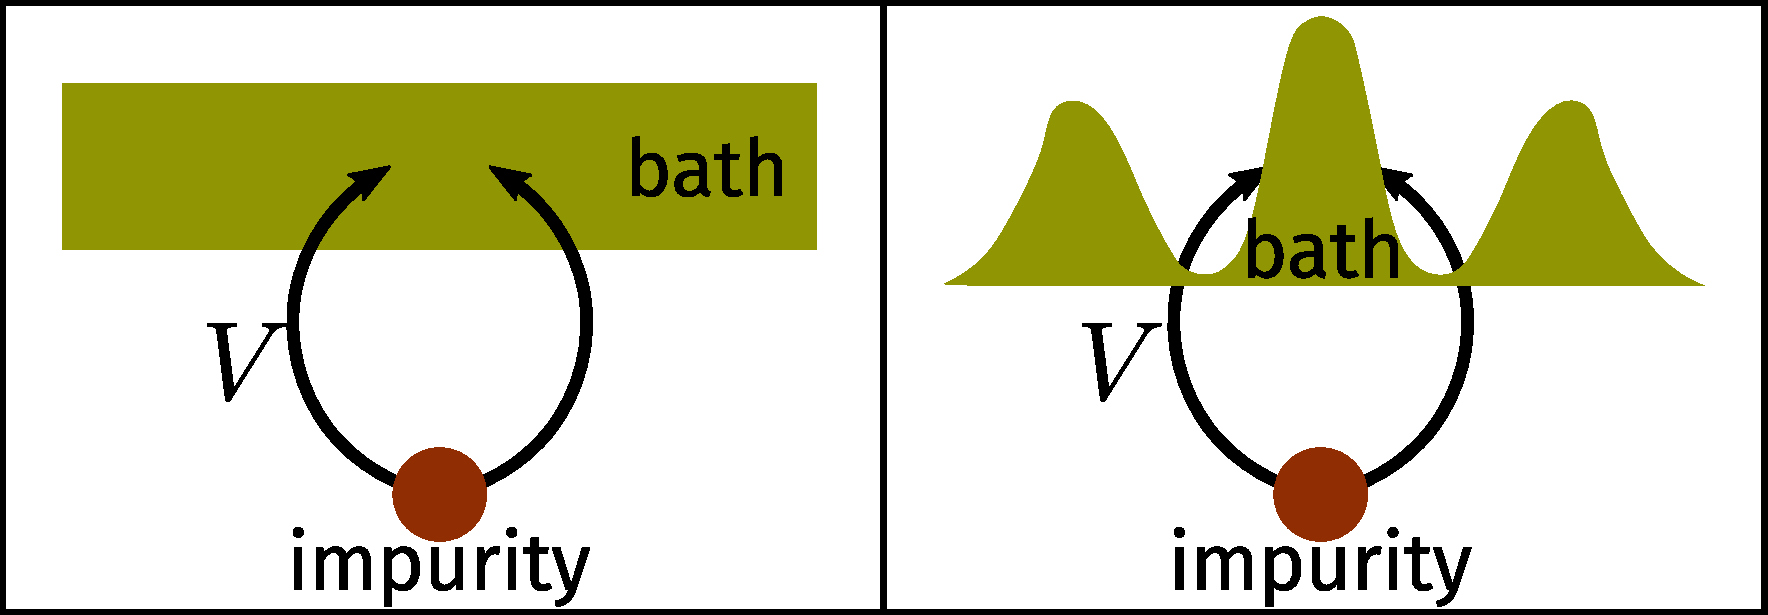
\includegraphics[width=0.5\textwidth]{../figures/dos_diff.pdf}
\caption{Various kinds of bath that an impurity can hybridise into. The left panel shows a non-interacting conduction band with a flat density of states. The right panel shows an interacting bath with an energy-dependent density of states. In the latter case, the impurity "feels" a reduced effective bandwidth defined by the width of the central peak.}
\end{figure}

\section{Summary of the Anderson impurity problem}
The single-impurity Anderson model (SIAM) is one of the most well-studied models in condensed matter physics and is the prototypical model for magnetism.
It shows how strong correlations can give rise to a residual local moment. Friedel\cite{}, in 1958, gave a phenomenological theory in which a local impurity developed an effective repulsion which forced the formation of bound states; those bound states where the up and down states became non-degenerate would correspond to the local moment.
Taking inspiration from this, P.W.Anderson\cite{anderson1970} in 1961 designed a model for the formation of local moment in second quantization.
The model consisted of a bath of mobile electrons which interacted with the local impurity.
The engine of magnetism was the local onsite Coulomb repulsion on the impurity site.
This repulsion favours the formation of local moments because it makes it harder for the impurity to be doubly-occupied.
 Mean-field calculations of the impurity occupation reveal a criterion for the formation of local moments; this criterion is similar to the Stoner criterion for ferromagnetism. This mean-field analysis is of course only valid at high temperatures where electron-correlations are not so important. At low temperatures, it was found that the resistivity of the material reaches a minimum at some temperature, and then increases as \(\ln T\) as we further reduce the temperature. This is in contrast to the previews results. And that was not all; at a sufficiently low temperature, it was found that the \(\ln T\)-dependence disappears and the susceptibility became constant, implying the formation of a singlet state.

 The fact that this logarithmic dependence vanishes once the singlet is formed suggests that it arises from the local moment on the impurity; once the local moment disappears (singlet), the log dependence vanishes as well.
This led people to design a model in which the impurity interacted with the conduction bath through a Heisenberg-like spin-spin interaction.
This model can be related to the SIAM through a canonical transformation followed by a projection to the low energy subspace\cite{schrieffer1966}.
In 1964, Jun Kondo\cite{kondo1964resistance,Zhang2013} found that a perturbative calculation of the transition probability of electrons from scattering via the impurity, up to second order in the exchange coupling \(J\), revealed a logarithmic dependence of the resistivity on temperature.
The crucial scattering process was that in which the spin of the incoming electron flipped (the \(S^+ s^-\) and \(S^- s^+\) terms).
This explained the mystery of the resistivity minimum and the logarithmic dependence.
But the mystery of the singlet state at very low temperatures still remained.
The perturbative analysis would break down at low temperatures, so it was unreliable.
The log term showed that the physics of the singlet involved all energy scales; one could not hope to capture it simply by taking the first few terms of a perturbative expansion.
This problem came to be known as the Kondo problem. 
Notable attempts to solve this problem include the Coulomb gas approach by Anderson and Yuval ~\cite{anderson1969exact,anderson1970exact}.
In 1970, Anderson attacked this problem by a renormalization group approach to account for all energy scales.
In his "Poor Man's Scaling" approach, he progressively reduced the bandwidth while taking account of the eliminated states into the couplings via second order perturbation theory. This showed how the couplings would flow as we went to low temperatures, but it still could not remove the divergence as it was perturbative.

Anderson found that the exchange coupling increased as we go to lower temperatures, so he surmised that the low energy theory was one where \(J=\infty\).
In 1975, Kenneth Wilson solved the problem by using his numerical renormalization group method in which he iteratively diagonalized chains of increasing length to go to the low energy physics~\cite{wilson1975,bullaNRGreview}.
He proved that Anderson's guess was right and the low energy Hamiltonian was the same as that with \(J=\infty\).
Later calculations with Bethe ansatz in 1980 by Andrei and Wiegmann \cite{andreiKondoreview,tsvelickKondoreview} corroborated Wilson's findings. Other methods like the conformal field theory~\cite{affleck1995conformal,affleck1993exact} and bosonisation~\cite{fradkin_1989} have also been applied to this problem.
Another important strong-coupling approach based on arguments of scattering phase shifts is that of the local Fermi liquid theory~\cite{nozieres1974fermi,nozaki2012} by Nozières. The low-temperature properties were found to be universal functions of a single energy scale, the Kondo temperature \(T_\text{K}\)~\cite{wilson1975,krishnamurthy-physrevlett.64.950,andreas_markus_2014,tadashi_1985,gass_kang_2011}.
All the predicted aspects of the Kondo effect, including the existence  of the Kondo cloud \cite{sorensen_erik_affleck_1996,affleck_ian_2001,simon_pascal_2003,martin2010,martin2019}, were observed experimentally in quantum dot systems~\cite{Goldhaber-Gordon1998,Cronenwett1998,Schmid_Weis1998,pustilnik_glazman_2004,Borzenets2020}. Scanning tunneling spectroscopy (STS) measurements have revealed that the Kondo effect often depends on the neighborhood of the impurities, in \(Cu\) and \(Co\) atoms~\cite{neel_berndt_2008,Zhao2005}.
It was also shown \cite{kaminski_nazarov2000}, using quantum dots, that the out of equilibrium Kondo effect also displays universality, the physics at low temperatures being decided by only two energy scales, the frequency and amplitude of the perturbation. 
The impurity spectral function has been calculated using NRG\cite{hrk_wilson_1980}, both at \(T=0\) \cite{sakai_osamu_shimizu,costi_hewson_1990} as well as \(T>0\) \cite{costi_kroha_wolfle}, as well as using diagrammatic methods \cite{kroha_wolfle}. 
The electrical resistivity was found to obey single-parameter scaling behavior in \(T/T_\mathrm{K}\) \cite{costi_hewson_1992}. 
Nozières went further and analyzed a more realistic model, the multi-channel Kondo problem in which multiple conduction bath channels interact with quantum impurity at the center \cite{Noz_blandin_1980}. 
Such a model was found, through methods like the Bethe ansatz, CFT and bosonization among others, to host a non-Fermi liquid low energy phase~\cite{Gan_Andrei_Coleman_1993,Noz_blandin_1980,emery_kivelson,Gan_mchannel_1994,Tsvelick_Weigmann_mchannel_1984,Tsvelick_weigmann_mchannel_1985,parcollet_olivier_large_N,kimura_taro_Su_N_kondo,PhysRevB.73.224445,cox_jarrell_two_channel_rev,affleck_1991_overscreen,Coleman_tsvelik}.
Kondo effect also occurs in light quark matter which interact with heavy quark impurities through gluon-exchange interactions; the scattering amplitude goes through a similar logarithmic divergence and renormalisation group calculations reveal a Kondo scale in such systems~\cite{Yasui_2013,hattori_2015}. Kondo effect can also be realized for other fermionic systems like graphene \cite{fritz_vojta_2013}, Dirac/Weyl semi-metals \cite{principi_2015,mitchell_lars_2015} and dense nuclear matter \cite{yasui_kazutaka_2017,yasui_shigehiro_2016,Yasui_2013}.


 A similar sequence of events also happened in the context of the Anderson model. In 1977 and 1978, Jefferson and Haldane independently calculated the "Poor Man's" scaling equations for the asymmetric SIAM, in the limit of infinitely large onsite repulsion. They were unable to access the strong-coupling fixed point (analogous to the \(J=\infty\) fixed point in Kondo model), but their equations revealed which were the important regimes to consider. Later, in 1975, Krishnamurthy, Wilkins and Wilson applied the NRG method to the symmetric Anderson model and obtained the non-perturbative fixed points and susceptibility \cite{hrk_wilson_1980}. Their calculations were again supported by later Bethe ansatz calculations by Wiegmann and Tsvelick\cite{tsvelickKondoreview}.
 The physics of the Anderson model and the Kondo model has connotations with quantum field theory. The numerical renormalization group methods ushered in a revolution. The idea that physics on all length scales affect the low energy physics was very deep and has far-reaching consequences. The phenomenon in which the impurity electron strongly couples to one real space lattice site at low temperatures resulting in the screening of the local moment via spin-flip scatterings with the mobile electrons at that site is analogous to the phenomenon of quark confinement in which the quarks become bound at low energies. The high energy fixed point, \(J=0\), corresponds to the phenomenon of asymptotic freedom in which the interactions between particles become asymptotically weaker at high temperatures.
\section{Some outstanding questions}
Even though the problem of the SIAM has been essentially solved, some questions and clarifications still remain. In this work, we explore some of these questions.
\begin{itemize}
    \item \textbf{Is it possible to get non-perturbative scaling equations for the whole journey?}

	    Neither NRG nor Bethe ansatz gives us scaling equations for the RG flows. Poor Man's scaling only gives perturbative ones which are valid close to the high energy theories. In the absence of scaling equations that show the complete crossover from the high energy to the low energy theory, it is difficult to visualize how the Hamiltonian is precisely chaining.

    \item \textbf{Is it possible to show the transfer of spectral weight along the flow, possibly by tracking the spectral function?}

	    Such an exercise will requite the entire spectrum to be preserved along the flow. NRG, being projective will not work here. If the entire spectrum is available, computing the spectral function along the flow should indicate how the spectral weight is being distributed between the impurity and the conduction bath, or between various states of the impurity. It can also shed light on which terms or processes in the Hamiltonian contribute to which parts of the spectral function.
    \item \textbf{How does NRG obtain the local moment in the absence of hybridisation?}
    For the symmetric mode, NRG results show that in the absence of any interaction between the bath and the impurity, the value of the onsite repulsion flows to a large value and we end up with a local moment. The obvious question is, how does the impurity coupling renormalize when there is no term connecting the bath with the impurity?
    \item \textbf{Are there any interesting topological aspects of the fixed points?}
	    We also intend to search for the existence of and possible changes in topological quantities at the fixed points. Since this is a zero-dimensional phenomenon, there will not be any gapping out of the Fermi surface, but there might be changes in topological quantities related to the Fermi surface or in the analyticity of the Green's function due to the presence of the coupling between the bath and the impurity. A strong indication of this is the change in the Wilson ratio from the non-interacting value of \(R=1\) to the local-Fermi liquid fixed point value of \(R=2\) obtained by Nozières\cite{nozieres1974fermi}. 
    \item \textbf{What is the nature of the Kondo cloud that screens the spin(charge) of the impurity?} We do not yet have a theory for the excitations of the cloud of electrons at the zeroth site that couple to the impurity at the fixed point. The local Fermi liquid sits just outside the cloud and is able to "feel" its effects and gauge certain gross quantities like the Wilson ratio, but it does not have the excitations of the cloud because that part, along with the impurity, has been assumed to be "frozen" into the singlet configuration. A recent result in this context \cite{anirban_kondo} is the effective Hamiltonian of the Kondo model cloud, also obtained using the same method that has been used in this thesis. The goal here is to do something similar for the SIAM as well.
    \item \textbf{How do entanglement measures respond to the RG flow?} Can we find a reflection of the screening mechanism in something like the mutual information or correlations? This requires a knowledge of the wavefunctions at the fixed point. Does the enhanced scattering of the electrons off the impurity lead to an increase in the entanglement between various electrons of the bath? It will also be interesting to check how various correlation functions vary across the RG flow.
\end{itemize}
\section{Salient features of the method}
The method employed in this work is a unitary renormalization group (URG) technique which progressively block-diagonalizes the Hamiltonian in the space of single high energy electrons. At each step of the process, the highest electron is decoupled from the system and it becomes an integral of motion, and the lower electronic system gets rotated to account for the decoupled electron. In this way, the RG goes on resolving the number fluctuations of the electrons. A fixed point is reached when the off-diagonal terms can no longer be removed. Since the method is unitary, it preserves the spectrum and allows calculating effective eigenvalues and eigenstates. It has some characteristic features:
\begin{itemize}
    \item \textit{Presence of a quantum fluctuation energy scale \(\omega\)}: 
The URG process involves a parameter \(\omega\) which contains the off-diagonal terms in the Hamiltonian. It quantifies the quantum fluctuation still unresolved in the system. Exactly at the fixed point, when the fluctuations are resolved, it assumes the value of one of the energies of the Hamiltonian. By probing the values of \(\omega\), all regions of the spectrum can, at least in principle, be accessed.
    \item \textit{Presence of finite-valued fixed points}:
The URG has a definite prescription for reaching the fixed point and it terminates after a finite number of steps (for a finite system). This leads to finite values of the fixed point  couplings. This is also in accordance with our intuition that finite systems should not have diverging couplings.
    \item \textit{Spectrum-preserving transformations}:
Since the RG transformations are unitary, all eigenvalues and eigenstates are kept track of the in the process. This allows us to calculate exact quantities for simple systems like the Kondo model.
    \item \textit{Tractable low-energy effective Hamiltonians}:
The final Hamiltonians obtained at the fixed point are usually tractable and allow us to extract information.
\end{itemize}

\section{Layout of the thesis}
Chapter \ref{prelims} goes over the available work on the single-impurity Anderson model and its derivative - Kondo model. We go over the mean-field calculation of the Anderson model which gives a criteria for magnetism in terms of the onsite repulsion parameter \(U\) and the hybridisation parameter \(\Delta\). We then derive the Kondo model from the SIAM by way of a Schrieffer-Wolff transformation, which we solve using NRG. We also spend some time on the Poor Man's scaling approaches of both the SIAM and the Kondo model, and end the chapter with some discussions on the local Fermi liquid aspects of the fixed point theory.

 Chapter \ref{urgform} lays out the URG formalism and prescription. We derive the URG effective Hamiltonian and the unitaries that perform the RG transformations. We discuss several important features of the method and provide a prescription for applying it on models. We also perform the URG explicitly on two models - the star graph model and the Kondo model. We discuss various subtleties, especially the quantum fluctuation parameter \(\omega\) and show that the URG actually diagonalizes the Hamiltonian. We derive many-body creation and annihilation operators \(\eta^\dagger\) and \(\eta\) which rotate the full Hamiltonian into successively more block-diagonal form.

 Chapter \ref{urg_canonical} is closely tied to the formalism chapter and develops the connections between URG and other canonical transformations in the literature. We first define and setup each of the other transformations - the Schrieffer-Wolff transformation (SWT), Poor Man's scaling (PMS) and the Continuous Unitary Transformation (CUT) RG. We show that all of these are in some sense perturbative derivatives of URG. A byproduct of the discussion is a demonstration of the fact that PMS and SWT are exactly identical and differ only in the contexts in which they are applied. We also discuss the differences between URG and CUT-RG, and show that URG behaves like a generalized double-bracket flow \cite{brockett_1991}. Chapter \ref{siamurg} contains the URG analysis of the standard SIAM, and it shows that such a model cannot display a phase transition and is hence not the appropriate auxiliary model for DMFT.

Chapter \ref{esiam-urg} contains the URG analysis of the extended SIAM, obtained by adding spin-spin and charge-charge interactions to the SIAM. The RG equations are derived in detail. We focus mostly on the generalised version. We discuss both the positive and the negative regimes of the impurity correlation \(U\). From the RG fixed point, we write down the fixed point Hamiltonian, and then discuss the spectrum of this Hamiltonian. We also compute some important quantities from the fixed point theory like the specific heat, magnetic susceptibility, charge susceptibility, Wilson ratio, Kondo cloud Hamiltonian, entanglement and correlation measures of the Kondo cloud electrons and change in the Luttinger's count of the bath. The Kondo cloud Hamiltonian is obtained by tracing out the impurity operators from the fixed point Hamiltonian. We compute the mutual information between between various members of the fixed point Hamiltonian, as well as some off-diagonal correlations. We extract a low temperature local Fermi liquid from the Hamiltonian which we then use to calculate the zero temperature Wilson ratio for the Kondo regime of the SIAM. We also calculate the change in Luttinger's volume between the fixed points.

Chapter~\ref{siam-attr-chap} contains the URG analysis of another extended SIAM obtained by adding an s-d coupling and an attractive local correlation in the bath. This model is shown to have a phase transition between local moment and singlet phases.

\section{Summary of main results}
The first of the main results in this work is the connection between URG and other canonical transformations. It is shown that URG is a non-perturbative variation of the most general unitary transformation. Other unitary transformations like the Schrieffer-Wolff transformation and Poor Man's scaling are simpler forms of URG, obtained by trivializing one of the terms in the Green's function that comes up in the URG formalism. CUT-RG is still more different from URG, since it is not only perturbative but also philosophically different in that it gradually suppresses the off-diagonal terms rather than killing more and more terms progressively. URG is thus different in two major ways - it provides non-perturbative equations because of the specific denominator structure as well as accommodates, at least in principle, the feedback effects of the off-diagonal terms through a quantum fluctuation operator in the denominator.
We next look at the results concerning the SIAM. In the absence of any spin-exchange or charge isospin-exchange scattering, we do not see any renormalization in the hybridisation and the only flow is towards a local moment fixed point with large impurity onsite energy \(U\). In the presence of those additional exchange scattering terms, the corresponding couplings \(J\)(spin exchange) and \(K\)(isospin exchange) flow to large values for low values of \(\omega\), signaling strong-coupling fixed points.
At the spin-screened strong-coupling fixed point (\(J>K\)), the ground state wavefunction is a superposition of a spin singlet and a charge-isospin triplet. The ground state for the isospin-dominated fixed point (\(K>J\)) is an isospin singlet. Thermodynamic quantities are now calculated using zero-mode Hamiltonians of the low energy effective theories. The impurity susceptibility \(\chi_\text{imp}\) goes to the Curie-Weiss value of a four-fold degenerate system at large temperatures, and becomes constant (paramagnetic) at very low temperatures. With \(T_K\) defined suitably, \(\chi_\text{imp}\) takes the zero temperature value of \(\left( 2\pi T_K \right) ^{-1}\). The impurity specific heat has also been calculated, and reveals a two-peak structure.
The fixed-point Hamiltonian further allows us to calculate the impurity spectral function. For very small \(U\) we obtain a single-peak structure corresponding to a single spin-spin or isospin-isospin excitation at the Fermi surface, while two other side-peaks emerge at large \(U\) that correspond to excitations between the spin and charge sectors. By tweaking the values of the couplings in the fixed-point Hamiltonian, we can mimic the reverse RG flow and see how the impurity spectral function morphs along this journey. Both the single-peak and three-peak structures revert back to a two-peak spectral function corresponding to that of a local moment.
We then extract the effective Hamiltonian for the Kondo cloud, up to two particle interactions, by tracing out the impurity from the coupled Hamiltonian. The Hamiltonian has both a Fermi liquid piece of the form \(\hat n_{k\sigma}\hat n_{q\sigma^\prime}\) and a two-particle off-diagonal scattering piece of the form \(c^\dagger_{k \uparrow}c^\dagger_{k^\prime \downarrow}c_{q \uparrow}c_{q^\prime \downarrow}\). It is the latter which is responsible for the screening mechanism. This conclusion is further strengthened by the studies of entanglement measures and correlations. The mutual information between the impurity and a cloud electron, as well as that between two cloud electrons increases as we go from the UV towards the IR fixed point. The off-diagonal correlation also increases from the UV towards the IR, which shows that the growth of the off-diagonal term is concomitant with the screening.
We also obtain the Wilson ratio of the impurity by creating a local Fermi liquid from the fixed point Hamiltonian. Using the zero charge susceptibility at \(T=0\) in the Kondo regime of the SIAM, we can show that the Wilson ratio goes to 2 at the fixed point. We also calculate the change in Luttinger's volume along the RG flow. At the free orbital or local moment fixed points, the Luttinger's volume is measured purely by the number of conduction electrons, but we see that at the strong-coupling fixed point, the correct Luttinger's volume is given by the total number of electrons in the conduction bath as well as the impurity. This is also connected to the increase in Wilson ratio from 1 to 2.
